\documentclass[a4paper,12pt,reqno]{amsart}
\usepackage{amsmath,amsfonts,amssymb}
\usepackage[usenames]{color}
\usepackage{tikz}
\usepackage{xcolor}
\usepackage{color}
\usetikzlibrary{arrows}

\begin{document}

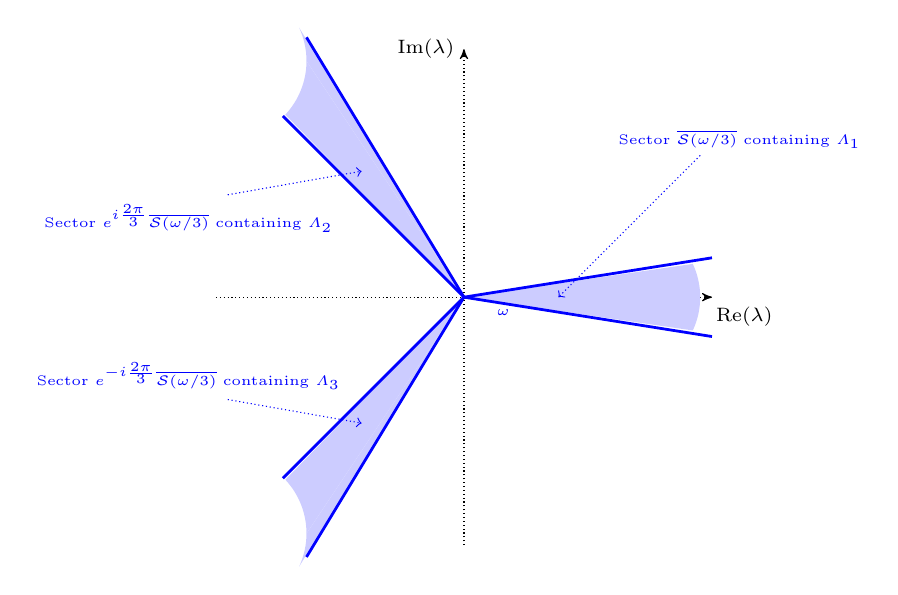
\begin{tikzpicture}
			\draw[-stealth', densely dotted] (-3.15,0) -- (3.15,0) node[below] {\ \ \ \ \ \ \ $\scriptstyle {\rm Re} (\lambda)$};
			\draw[-stealth', densely dotted ] (0,-3.15) -- (0,3.15) node[left] {\color{black}$\scriptstyle{\rm Im} (\lambda)$};
			%%%%%%%%%%%%%%%%%%%%%%%%%%%%%%%%%%%%%%%%%%%%%%%%%%%%
			\fill[blue!20!] (0,0) -- (3,0) arc (0:25:1cm)-- cycle;
			\fill[blue!20!] (0,0) -- (3,0) arc (0:-25:1cm)-- cycle;
			%%%%%%%%%%%%%%%%%%%%%%%%%%%%%%%%%%%%%%%%%%%%%%%%%%%%%%%%%
			\fill[blue!20!] (0,0) -- (-2,3) arc (0:25:1cm)-- cycle;
			\fill[blue!20!] (0,0) -- (-2,3) arc (0:-43:1cm)-- cycle;
			%%%%%%%%%%%%%%%%%%%%%%%%%%%%%%%%%%%%%%%%%%%%%%%%%%%%%%%%%%%
			%%%%%%%%%%%%%%%%%%%%%%%%%%%%%%%%%%%%%%%%%%%%%%%%%%%%%%%%%
			\fill[blue!20!] (0,0) -- (-2,-3) arc (0:-25:1cm)-- cycle;
			\fill[blue!20!] (0,0) -- (-2,-3) arc (0:43:1cm)-- cycle;
			%%%%%%%%%%%%%%%%%%%%%%%%%%%%%%%%%%%%%%%%%%%%%%%%%%%%%%%%%%%
			\node at (3.5,2) {{\tiny\color{blue} Sector $\overline{\mathcal{S}(\omega/3)}$ containing  $\varLambda_1$}};
			\node at (-3.5,1) {{\tiny\color{blue} Sector  $e^{i\frac{2\pi}{3}}\overline{\mathcal{S}(\omega/3)}$ containing  $\varLambda_2$}};
			\node at (-3.5,-1) {{\tiny\color{blue} Sector $e^{-i\frac{2\pi}{3}}\overline{\mathcal{S}(\omega/3)}$ containing  $\varLambda_3$}};
			
			%%%%%%%%%%%%%%%%%%%%%%%%%%%%%%%%%%%%%%%%%%%%%%%%
			\draw[color=blue,->, densely dotted] (-3,1.3) -- (-1.3,1.6);
			\draw[color=blue,->, densely dotted] (-3,-1.3) -- (-1.3,-1.6);
			\draw[color=blue,->, densely dotted] (3,1.8) -- (1.2, 0);
			%%%%%%%%%%%%%%%%%%%%%%%%%%%%%%%%%%%%%%%
			\draw[color=blue, line width=1pt] (3.15,0.5) -- (0,0);
			\draw[color=blue, line width=1pt] (3.15,-0.5) -- (0,0);
			%%%%%%%%%%%%%%%%%%%%%%%%%%%%%%%%%%%%%%%%%%%%%%%%%%%%%%%%%%
			\draw[color=blue, line width=1pt] (-2, 3.3) -- (0,0);
			\draw[color=blue, line width=1pt] (-2.3, 2.3) -- (0,0);
			%%%%%%%%%%%%%%%%%%%%%%%%%%%%%%%%%%%%%%%%%%%%%%%%%%%%%%
			\draw[color=blue, line width=1pt] (-2, -3.3) -- (0,0);
			\draw[color=blue, line width=1pt] (-2.3, -2.3) -- (0,0);
			%%%%%%%%%%%%%%%%%%%%%%%%%%%%%%%%%%%%%%%%%%%%%%%%%%%%%%%%%
			\node at (0.5,-0.2) {\color{blue}{\tiny $\omega$}};
		\end{tikzpicture}

\end{document}